%%%%
% Consiglio la visione dei seguenti tutorial:
% - https://www.youtube.com/watch?v=ihxSUsJB_14
% - https://www.youtube.com/watch?v=XTFWaV55uDo
%%%%
\documentclass[12pt,a4paper,openright,twoside]{book}
\usepackage[utf8]{inputenc}
\usepackage{float}
\usepackage{hyperref}
\usepackage{caption}
\usepackage{subcaption}

\newcommand{\thesislang}{italian} % decommentare in caso di tesi in italiano
%\newcommand{\thesislang}{english} % commentare in caso di tesi in italiano
\usepackage{thesis-style}

\begin{document}
	
\frontmatter

% ! TeX root = thesis-main.tex
\title{Title}
\author{Candidate Name Here}
\date{\today}

\begin{titlepage}
	\begin{center}
		% \vspace*{0.2cm}
		
		\large
		\textbf{ALMA MATER STUDIORUM -- UNIVERSITÀ DI BOLOGNA \\ CAMPUS DI CESENA}
		\\
		\noindent\hrulefill
		\vspace{0.4cm}
		
		\Large
		Scuola di Ingegneria e Architettura \\
		Corso di Laurea Magistrale in Ingegneria e Scienze Informatiche
		
		\Huge
		\vspace{4cm}
		\textbf{Assignment \#03}
		
		\large
		\vspace{1cm}
		Elaborato in 
		\\
		\textsc{Programmazione concorrente e distribuita}
		
		\vspace{5.5cm}
		\begin{minipage}[t]{0.64\textwidth}
			\begin{flushleft}
			\end{flushleft}
		\end{minipage}
		\begin{minipage}[t]{0.34\textwidth}
			\begin{flushright}
				\textit{Studenti} 
				\\ 
				\textbf{Eddie Barzi}
				\\ 
				\textbf{Filippo Vissani}
			\end{flushright}
		\end{minipage}\\
		
		\vfill
		\noindent\hrulefill
		\vspace{0.3cm}
		\Large

		Anno Accademico 2021-2022
	\end{center}
\end{titlepage}
\restoregeometry


%----------------------------------------------------------------------------------------
\tableofcontents   
%\listoffigures     % (optional) comment if empty
%\lstlistoflistings % (optional) comment if empty
%----------------------------------------------------------------------------------------

\mainmatter

%----------------------------------------------------------------------------------------
\chapter{\introductionname}
\label{chap:introduction}
%----------------------------------------------------------------------------------------
\section{Descrizione e Obiettivi}
\subsection{Actor Programming}
Viene fornito il codice di un programma che simula il movimento di $N$ corpi su un piano bidimensionale,
soggetti a due tipi di forze:
\begin{itemize}
	\item una forza repulsiva, per cui ogni corpo $b_{i}$ esercita su ogni altro corpo $b_{j}$ una forza in modulo pari a:
	\begin{center}
		$ F_{ij} = \frac{k_{rep} \times m_{i}}{d^2_{ij}} $
	\end{center}
	Dove $m_{i}$ è la massa del corpo $b_{i}$, $k_{rep}$ è una costante data, $d_{ij}$ è la distanza fra i due corpi.
	La direzione della forza è data dal versore $(b_{i} - b_{j})$, ovvero respingente per il corpo $b_{j}$.
	\item Una forza di attrito, per cui su ogni corpo $b_{i}$ che si muove a una velocità $v_{i}$ è esercitata una forza:
	\begin{center}
		$ FR_{i} = - k_{fri} \times v_{i} $
	\end{center}
	Che si oppone al moto, quindi in direzione opposta alla sua velocità, dove $k_{fri}$ è una costante data.
\end{itemize}
Il programma è sequenziale, non strutturato. 
L'algoritmo \ref{lst:lst1} definisce il comportamento del simulatore in pseudo codice.
\newpage
\begin{lstlisting}[label=lst:lst1,caption=Pseudocodice del programma sequenziale]
/* virtual time */
vt = 0;
/* time increment at each iteration */     
dt  = 0.01;

loop:
	for each body b[i]:
		compute total force exerted by other bodies b[j] and friction;
		compute the instant acceleration, given the total force and mass;
		update body velocity, given the acceleration and the virtual time elapsed dt;
	update bodies positions, given the velocity and virtual time elapsed dt;
	check boundary collisions;
	vt = vt + dt;   
	display current stage;

\end{lstlisting}

Alcuni aspetti rilevanti in merito al comportamento del programma e alla natura del problema:
\begin{itemize}
	\item Il calcolo delle forze al tempo $t$ avviene considerando coerentemente le posizioni dei corpi al tempo $t$. 
	\item L'aggiornamento delle posizioni può avvenire solo dopo che tutte le forze sono state calcolate (e le velocità aggiornate).
	\item Il controllo della collisione con i confini del mondo per un corpo $b_{i}$ può comportare il cambiamento della velocità e posizione del corpo.
	\item Nel programma, la visualizzazione dello stato corrente della simulazione o frame (via GUI) avviene in modo sincrono, per cui la successiva iterazione avviene solo dopo aver visualizzato lo stato della precedente.
\end{itemize}

Si vuole realizzare una versione orientata agli attori della simulazione senza GUI, considerando un insieme iniziale $N$ di corpi
- e calcolando l'evoluzione temporale per un certo numero di passi $Nsteps$ -
con $Nsteps$ fissato come parametro. Posizione e velocità iniziali possono essere definite in modo casuale.

Inoltre si voglio paragonare i risultati ottenuti con quelli degli assignment precedenti.

Estendere la simulazione includendo una GUI con pulsanti start/stop per lanciare/fermare la simulazione e visualizzare l'andamento,
includendo informazioni circa il tempo virtuale.
La GUI si presuppone visualizzi stati consistenti della simulazione (ma non necessariamente tutti gli stati).

%----------------------------------------------------------------------------------------

\subsection{Distributed Programming}
Si vuole creare un’applicazione distribuita che ha lo scopo di monitorare possibili allagamenti in una smart-city. Per questo obiettivo, nella città vengono installati un certo numero (prefissato) di “smart thing” che percepiscono alcuni dati ambientali. In particolare, diversi pluviometri hanno l’obiettivo di controllare il livello di pioggia caduta (espressa in mm3) in un certo intervallo di tempo. Un pluviometro è collocato in una certa posizione (per semplicità, in uno spazio piano di due dimensioni). La città è divisa in zone (predefinite) e ogni pluviometro opera in una sola zona. Per semplicità, l’area della città viene considerata come un rettangolo WxH collocato in uno spazio euclideo (Figura \ref{fig:dpc}).
\begin{figure}[H]
	\centering
	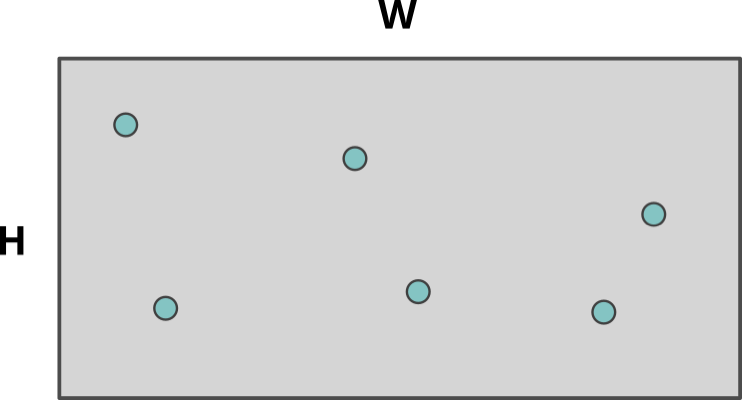
\includegraphics[width=\textwidth]{figures/distributed-programming-city.png}
	\caption{Distributed Programming: l’area della città viene considerata come un rettangolo WxH.}
	\label{fig:dpc}
\end{figure}
Le zone devono coprire completamente l’area della città, non può esistere una porzione dello spazio non gestita dal sistema o appartenente a due zone (Figura \ref{fig:dpd}). 
\begin{figure}[H]
	\centering
	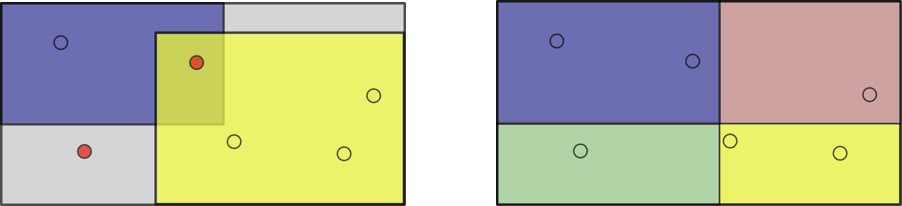
\includegraphics[width=\textwidth]{figures/distributed-programming-division.png}
	\caption{Distributed Programming: divisione in zone sbagliata a sinistra e corretta a destra.}
	\label{fig:dpd}
\end{figure}
Per semplicità, in questo caso si suppone che il rettangolo sia suddiviso seguendo una griglia CxR (Figura \ref{fig:dpg}). Si possono considerare divisioni spaziali in base al numero di zone (e.g., ogni area può contenere al massimo tre dispositivi).
I pluviometri devono andare in una condizione di allarme quando la maggioranza dei sensori in una certa zona percepisce un valore sopra a una certa soglia (prefissata).
Anche se il numero totale di pluviometri è fissato, ognuno di essi può fallire, quindi la maggioranza per una certa zona può cambiare nel tempo.
\begin{figure}[H]
	\centering
	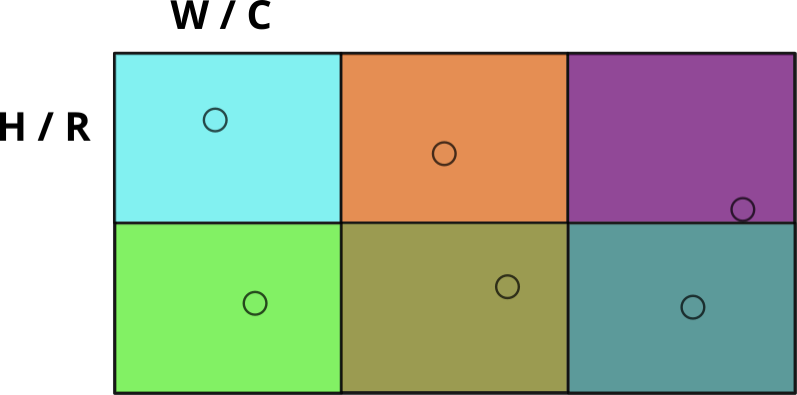
\includegraphics[width=\textwidth]{figures/distributed-programming-grid.png}
	\caption{Distributed Programming: suddivisione del rettangolo seguendo una griglia CxR.}
	\label{fig:dpg}
\end{figure}
Quando la zona è in allarme, il sistema deve allertare una delle caserme dei pompieri vicina all’allarme generato. Una stessa caserma può al massimo gestire un allarme. Per semplicità, ogni zona ha una caserma dei pompieri.
L’allarme generato dai sensori può essere disabilitato solamente da una caserma di pompieri (quindi anche se le percezioni ritornano sotto soglia, l’allarme di una certa zona deve restare attivo).
Infine, i pompieri hanno accesso a un'applicazione (con GUI) tramite con cui è possibile:
\begin{itemize}
    \item visualizzare lo stato delle zone (ok/allarme/in gestione)
    \item visualizzare il numero di sensori in una certa zona
    \item visualizzare lo stato delle caserme (libera, occupata)
    \item disabilitare allarmi
\end{itemize}
La soluzione deve essere peer-to-peer (basata su attori oppure può sfruttare un MOM).
\chapter{Analisi del Problema}
\label{chap:Analisi del Problema}
%----------------------------------------------------------------------------------------
\section{Actor Programming}
Introducendo la programmazione ad attori nel programma devono essere considerati i seguenti aspetti:
\begin{itemize}
	\item La rappresentazione della simulazione deve rimanere
	consistente, gli attori che gestiscono i corpi devono essere sempre sincronizzati sulla stessa iterazione.
	\item Gli eventi relativi alla pressione dei pulsanti
	devono essere gestiti atomicamente, dato che si occupano di
	avviare e fermare i flussi di esecuzione.
	\item I singoli attori non devono eseguire computazioni onerose in termini di tempo, il carico di lavoro deve essere adeguatamente distribuito.
\end{itemize}


%----------------------------------------------------------------------------------------

\section{Distributed Programming}
Il primo problema da considerare è quello della divisione in zone senza sovrapposizioni e aree vuote. Per questo è conveniente considerare le suddivisioni sempre seguendo la griglia CxR. Quindi, considerando anche che una zona può avere al massimo tre pluviometri e che il numero di pluviometri è fissato a sei, si possono avere da un minimo di due a un massimo di sei zone. Ogni zona deve essere definita da dei limiti spaziali che stabilisco anche la sua posizione all'interno della città.

L'assegnamento dei sei pluviometri deve essere gestito correttamente, gestendo tutte le casistiche descritte per le zone. Non devono essere presenti zone senza pluviometri e all'interno di una zona non possono essere presenti più di tre pluviometri. Bisogna anche considerare i casi in cui le zone non hanno lo stesso numero di pluviometri; ad esempio, con quattro zone si ottengono due zone con due pluviometri e altre due zone con un pluviometro.

All'interno di una zona troviamo attori con comportamenti differenti, è fondamentale che ogni attore comunichi correttamente con gli altri presenti nella sua zona e non invii per errore messaggi ad attori di altre zone. Per rispettare questo vincolo è necessario assegnare un identificativo univoco ad ogni zona e implementare una procedura che permetta ad ogni attore di recuperare i riferimenti corretti al suo avvio.

Dato che il sistema deve essere peer-to-peer, non è possibile creare un punto centralizzato che detiene tutte le informazioni, quindi i pluviometri devono stabilire se la zona è in allarme comunicando tra loro. Qui sorge la necessità di stabilire un protocollo di comunicazione tra i pluviometri che permetta di contattare la stazione solo in caso di necessità. Nell'implementare tale protocollo bisogna tenere conto del fatto che un pluviometro può fallire e quindi non rispondere ad una determinata richiesta. Volendo proporre una prima soluzione a questo problema, ogni volta che un pluviometro invia la richiesta agli altri considera solo le risposte che arrivano entro un lasso di tempo prestabilito, in questo modo è possibile rilevare in modo dinamico se la maggior parte dei pluviometri è in allarme, quindi non considerando quelli non raggiungibili.
\chapter{Descrizione dell'Architettura Proposta}
\label{chap:Descrizione dell'Architettura Proposta}
%----------------------------------------------------------------------------------------
\section{Actor Programming}
In fase di progettazione si è scelto di impiegare una versione ad attori del pattern architetturale \textit{Model-View-Controller}, in cui View, Controller e Model vengono considerati come attori (Figura \ref{fig:apmvc}).
Mentre al Controller e alla View corrisponde un singolo attore che gestisce il componente, per il model si è scelto di considerare ogni corpo come un attore.
L'attore Root si occupa di generare gli attori che gestiscono View, Controller e corpi (Figura: \ref{fig:apc}) e di far partire la simulazione (nel caso in cui la GUI non sia presente).

Il comportamento del sistema viene descritto in Figura (Figura: \ref{fig:api})
All'avvio della simulazione il ControllerActor richiede lo stato a tutti i BodyActor, che rispondono come specificato nel pattern Request-Response. Una volta ricevuto lo stato di tutti i corpi, il Controller ha a disposizione un'immagine dell'iterazione corrente della simulazione, che replica su tutti i corpi. A questo punto i corpi possono aggiornare la loro posizione sfruttando lo stato dell'iterazione precedente.
Una volta aggiornata la posizione, i corpi inviano nuovamente il loro stato al Controller, il quale, dopo ricevuto il nuovo stato di tutti i corpi, lo replica sulla View contattando l'attore che la gestisce.
La \textit{View} (Figura \ref{fig:apgui}) oltre a rappresentare lo stato corrente della simulazione, riporta il tempo virtuale e l'iterazione correnti.
L'interfaccia grafica dispone di quattro pulsanti:
\begin{itemize}
    \item Start: per avviare la simulazione
    \item Stop: per fermare la simulazione
    \item Zoom In: per aumentare lo zoom della simulazione
    \item Zoom Out: per diminuire lo zoom della simulazione
\end{itemize}
\begin{figure}[H]
	\centering
	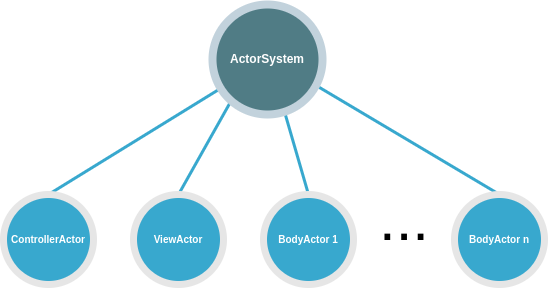
\includegraphics[width=\textwidth]{figures/actor-programming-mvc.png}
	\caption{Actor Programming: Model-View-Controller.}
	\label{fig:apmvc}
\end{figure}
\begin{figure}[H]
	\centering
	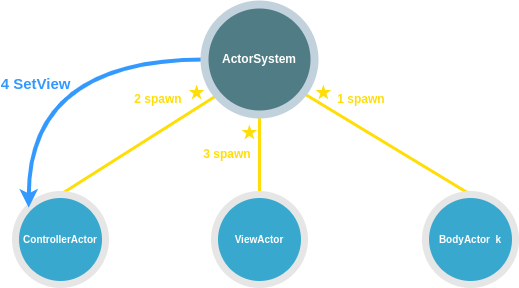
\includegraphics[width=\textwidth]{figures/actor-programming-creation.png}
	\caption{Actor Programming: creazione degli attori.}
	\label{fig:apc}
\end{figure}
\begin{figure}[H]
	\centering
	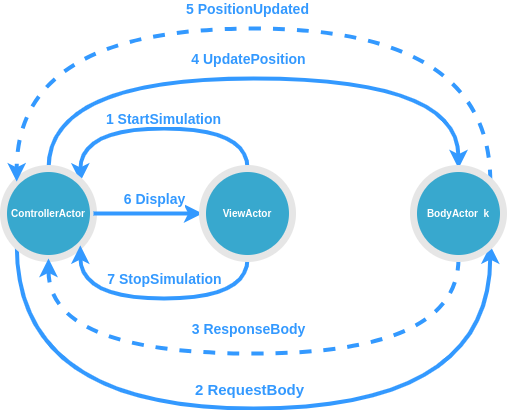
\includegraphics[width=\textwidth]{figures/actor-programming-interaction.png}
	\caption{Actor Programming: interazioni tra attori.}
	\label{fig:api}
\end{figure}
\begin{figure}[H]
	\centering
	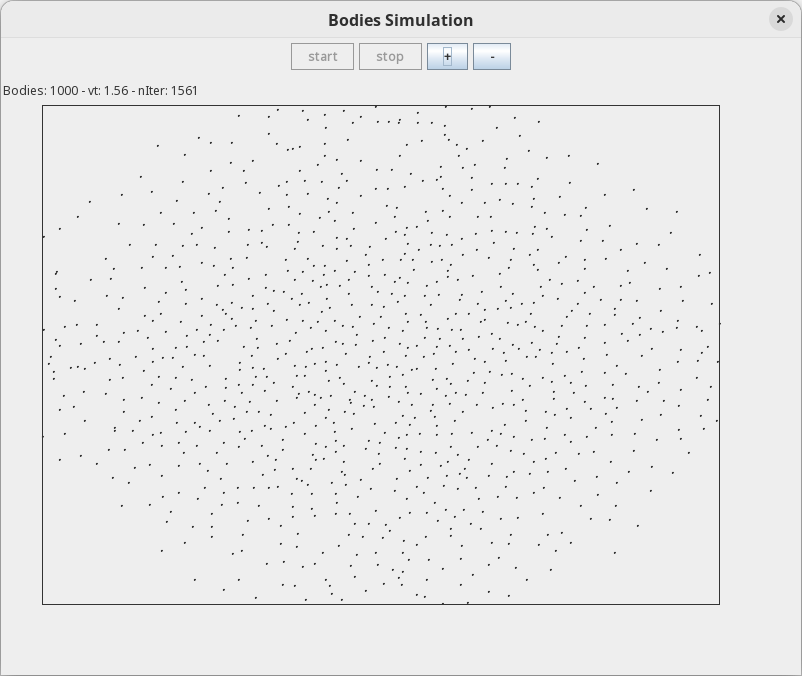
\includegraphics[width=\textwidth]{figures/actor-programming-simulation.png}
	\caption{Actor Programming: interazioni tra attori.}
	\label{fig:apgui}
\end{figure}

%----------------------------------------------------------------------------------------
\subsection{Verifica delle Prestazioni}
%----------------------------------------------------------------------------------------
La macchina su cui sono stati effettuati i test ha le seguenti caratteristiche:
\begin{itemize}
	\item Sistema operativo: Fedora 36 (GNU/Linux)
	\item Desktop environment: Gnome 42.2
	\item Versione kernel Linux: 5.18.6
	\item Memoria: 16GB, 3200Mhz
	\item CPU: AMD Ryzen 7 5700U
\end{itemize}
Descrizione dettagliata del processore:
\begin{itemize}
	\item Core: 8
	\item Thread: 16
	\item Clock base: 1.8GHz
	\item Clock max: 4.3GHz
	\item Cache L2: 4MB
	\item Cache L3: 8MB
\end{itemize}

Nella tabella \ref{tab:table1} vengono riportati i risultati dei test effettuati usando Monitor, Java Executor e Attori. Lo speedup non è presente perché non è stato possibile stabilire a priori il numero di worker nella programmazione ad attori.
Dalla tabella risulta che l'approccio di programmazione con gli Executor è più efficiente rispetto agli altri, soprattutto rispetto a quello che fa uso degli attori.

\begin{table}[h!]
	\centering
	\begin{tabular}{ |c|c|c|c|c|c| } 
	\hline
    &&& \multicolumn{3}{|c|}{Tempo esecuzione (ms)} \\
    \hline
	N° & Corpi & Iterazioni & Monitor & Executor & Attori \\
	\hline
	0 & 100 & 1000 & 0h0m0s638ms & 0h0m0s198ms & 0h0m6s618ms \\ 
    \hline
    1 & 100 & 10000 & 0h0m6s265ms & 0h0m1s950ms & 0h1m5s549ms \\ 
     \hline
    2 & 100 & 50000 & 0h0m41s122ms & 0h0m12s43ms & 0h6m47s6ms \\ 
     \hline
    3 & 1000 & 1000 & 0h0m4s626ms & 0h0m4s24ms & 0h1m35s593ms \\ 
     \hline
    4 & 1000 & 10000 & 0h0m45s522ms & 0h0m40s143ms & 0h15m16s555ms \\ 
     \hline
    5 & 1000 & 50000 & 0h3m50s52ms & 0h3m21s167ms & 1h22m2s171ms \\ 
     \hline
    6 & 5000 & 1000 & 0h1m35s518ms & 0h1m34s657ms & 0h11m2s895ms \\ 
     \hline
    7 & 5000 & 10000 & 0h15m56s272ms & 0h15m38s990ms & 1h53m25s264ms \\ 
     \hline
    8 & 5000 & 50000 & 1h20m1s527ms & 1h19m23s385ms & 9h30m34s389ms \\ 
     \hline
	\end{tabular}
	\caption{Actor Programming: Comparativa dei risultati ottenuti con i diversi approcci.}
	\label{tab:table1}
\end{table}

\section{Distributed Programming}
All'avvio, il programma prende in input la dimensione della città (WxH) e il numero di righe e di colonne in cui suddividerla (CxR). È possibile generare da un minimo di due a un massimo di sei zone, i pluviometri vengono assegnati automaticamente. Le posizioni della stazione e dei pluviometri vengono stabilite in modo casuale all'interno della loro zona di appartenenza.
All'interno del sistema troviamo sei tipi di attori, che vengono utilizzati per modellare gli aspetti riguardanti i sensori, le stazioni dei pompieri e l'interfaccia grafica.

PluviometerActor e PluviometerGuardianActor vengono utilizzati per la gestione dei pluviometri e fanno parte dello stesso actor system. In particolare, PluviometerGuardianActor genera PluviometerActor ed esegue la sottoscrizione ai servizi forniti dagli altri pluviometri, dalle stazioni e dalle interfacce grafiche. Questa procedura viene eseguita sfruttando la funzionalità Receptionist fornita da Akka.
Ogni PluviometerActor, al suo avvio registra il servizio che rende disponibili i suoi messaggi all'interno del cluster e inizializza un timer periodico di cinque secondi. Ogni volta che il timer di un PluviometerActor si resetta, questo richiede agli altri pluviometri della sua zona se sono in allarme, se la maggior parte dei pluviometri della zona risulta in allarme allora il pluviometro che ha inviato la richiesta contatta la stazione dei vigili del fuoco. Siccome i pluviometri possono fallire, questa procedura viene eseguita rispettando il pattern Ask, quindi la risposta viene attesa per un massimo di due secondi; se un pluviometro non risponde ad una richiesta viene considerato non raggiungibile.

FireStationActor e FireStationGuardianActor vengono utilizzati per la gestione delle stazioni e fanno parte dello stesso actor system. Al loro avvio, si comportano allo stesso modo di PluviometerActor e PluviometerGuardianActor rispettivamente, per quanto riguarda la registrazione e la sottoscrizione dei servizi.
FireStationActor può essere avvisato da uno dei pluviometri della zona e può essere contattato da un ViewActor per gestire e sistemare la zona. In particolare, ai seguenti stati della zona corrispondono i rispettivi stati del FireStationActor:
\begin{table}[h!]
	\centering
	\begin{tabular}{ |c|c| }
    \hline
	\textbf{Stato Zona} & \textbf{Stato Stazione} \\
	\hline
	Ok & Free \\
	\hline
	Alarm & Warned \\
	\hline
	UnderManagement & Busy \\
	\hline
	\end{tabular}
\end{table}

ViewGuardianActor e ViewActor vengono utilizzati per la gestione dell'interfaccia grafica, anche in questo caso i due attori fanno parte dello stesso actor system e il loro comportamento iniziale è simile a quelli descritti precedentemente, per quanto riguarda la gestione dei servizi.
ViewActor gestisce l'interfaccia grafica (Figura \ref{fig:dpgui}) che permette di visualizzare lo stato delle zone della città e di gestire la zona assegnata nel caso in cui sia in allarme o in gestione.
\begin{figure}
     \centering
     \begin{subfigure}[b]{0.3\textwidth}
         \centering
         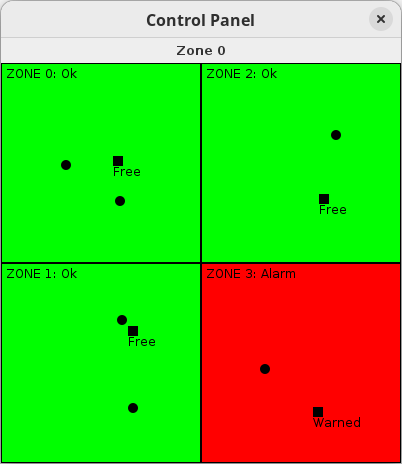
\includegraphics[width=\textwidth]{figures/distributed-programming-gui-ok.png}
         \caption{Ok}
         \label{fig:dpguia}
     \end{subfigure}
     \hfill
     \begin{subfigure}[b]{0.3\textwidth}
         \centering
         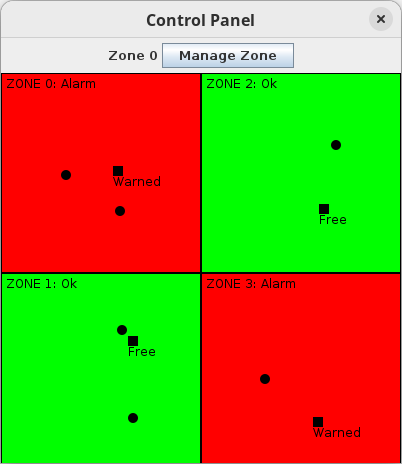
\includegraphics[width=\textwidth]{figures/distributed-programming-gui-alarm.png}
         \caption{Allarme}
         \label{fig:dpguib}
     \end{subfigure}
     \hfill
     \begin{subfigure}[b]{0.3\textwidth}
         \centering
         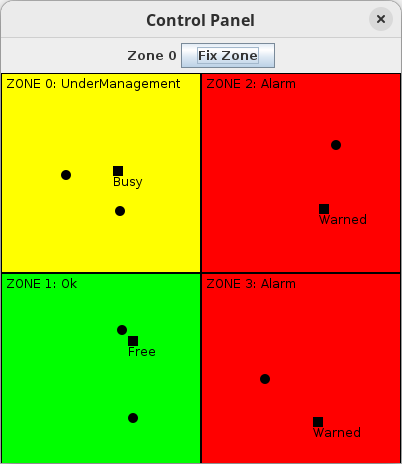
\includegraphics[width=\textwidth]{figures/distributed-programming-gui-management.png}
         \caption{In gestione}
         \label{fig:dpguic}
     \end{subfigure}
        \caption{Distributed Programming: Interfaccia grafica}
        \label{fig:dpgui}
\end{figure}

Il comportamento degli attori viene descritto più nel dettaglio in Figura \ref{fig:dpai1} e in Figura \ref{fig:dpai2}.

\begin{figure}
	\centering
	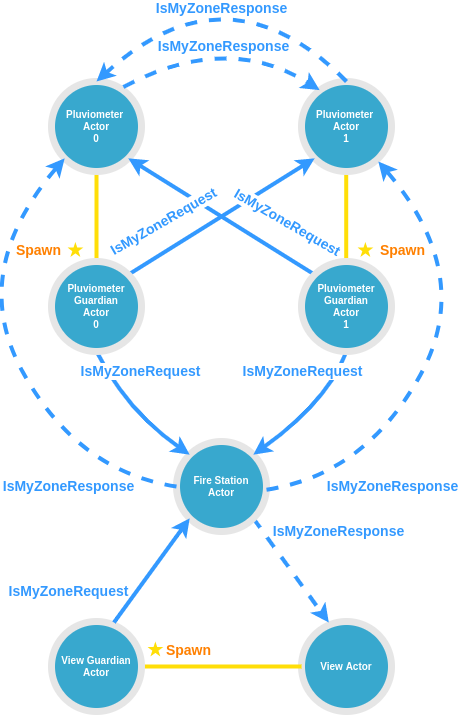
\includegraphics[width=0.7\textwidth]{figures/distributed-programming-actors-interactions1.png}
	\caption{Distributed Programming: interazioni tra attori all'avvio.}
	\label{fig:dpai1}
\end{figure}

\begin{figure}
	\centering
	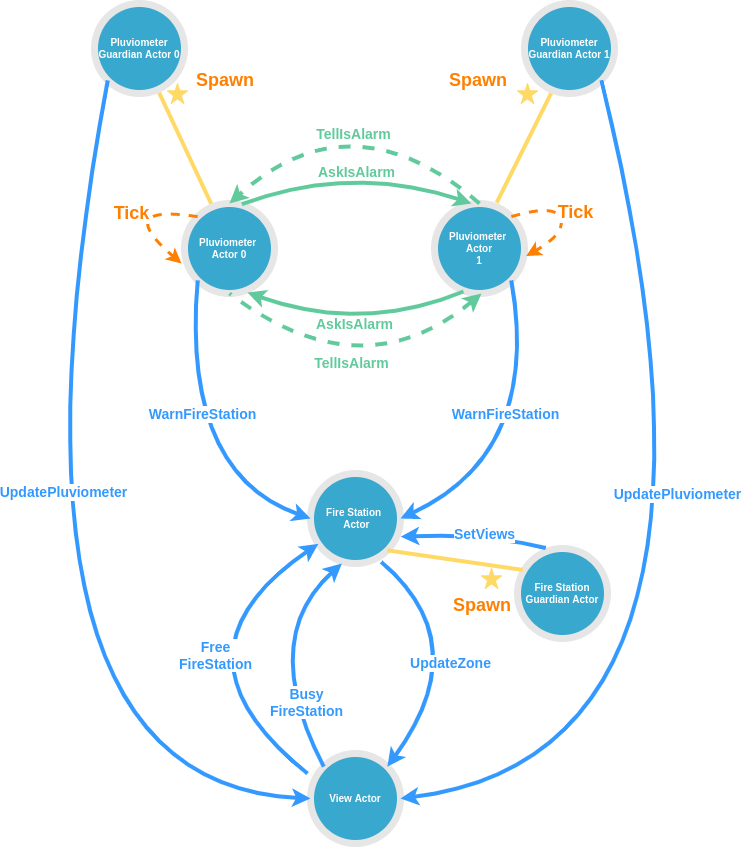
\includegraphics[width=\textwidth]{figures/distributed-programming-actors-interactions2.png}
	\caption{Distributed Programming: interazioni tra attori.}
	\label{fig:dpai2}
\end{figure}

\end{document}